\chapter{真实大规模场景数据下的混合隐式场学习}
\label{chapter: real-world data}
\section{基于时间-位姿隐式场的多元传感信息配准}
大规模场景的混合隐式表达对于真实场景中地图重建是自动驾驶、无人机运输等智能交通应用的下一代地图表征工具。然而对于大规模场景的多元传感数据的同步采集,现有的同步RGB-D相机因其可以感知到的深度范围及其有限,从而不能被直接应用,而使用不同步的RGB相机和深度传感器(激光雷达等)不可避免的需要解决其中的时钟同步问题。受近期的自动标定相机内外参数的的神经隐式场方法所启发,本文提出了首个自动标定RGB相机和深度传感器间采样频率和偏置的解决方案。

本文利用了一个重要的领域先验,即同时搭载不同种类传感器的数据采集设备在时空上覆盖了几乎完全相同的行动轨迹,提出建模时间到位姿的隐式函数关系。本文的方法可以作为第\ref{chapter: omninerf}章中混合隐式场景表示模型的前置网络,提供较为准确的位姿数据。

近年来,神经隐式表达被广泛用于大规模场景的隐式重建中\cite{tancik_block-nerf_2022, rematas_urban_2022, turki_mega-nerf_2022, xiangli_bungeenerf_2022},由于此类方法通常具有较好的新视角渲染能力,他们通常被看作下一代视觉导航系统中的地图表示模型。不妨想象,在未来,同时定位与建图(Simultaneously Localization and Mapping, SLAM)系统可以快速整合不同种类的传感信息,构建准确的基于神经隐式场的地图表示\cite{zhu_nice-slam_2022, zhu_nicer-slam_2023, sandstrom_point-slam_2023},场景图(SceneGraph)算法可以通过车端RGB相机和消费级激光雷达快速构建周边区域的动态场景图,准确对路端中行人、机动车的未来轨迹进行预测\cite{ost_neural_2021, kundu_panoptic_2022, yang_urbangiraffe_2023, , chen_geosim_2021}。

然而,目前的这些方法仍然没有系统性地解决使用深度数据作为有效监督信号的一个关键问题。使用深度图作为监督信号加入到神经隐式表达的训练过程听起来是一个非常浅显易懂的概念,然而这一概念在真实大场景数据获取、使用上存在着相当复杂的时间同步问题。本文注意到市面上使用较为广泛的RGB-D同步相机如微软Kinect相机\cite{zhang_microsoft_2012}、英特尔RealSense相机\cite{, zabatani_intel_2020}等通常只能感知到受限范围内(通常在5米以内)的物体,从而只能用于室内场景的数据获取中,而不能用于更加广泛的室外场景自动驾驶、无人机运输等智能交通算法中。 另一方面,使用异步的 RGB 和深度传感器会带来更多的复杂性,因为这通常意味着需要估计每个RGB帧和深度帧之间的转换矩阵。

\begin{figure}[ht]
    \centering
    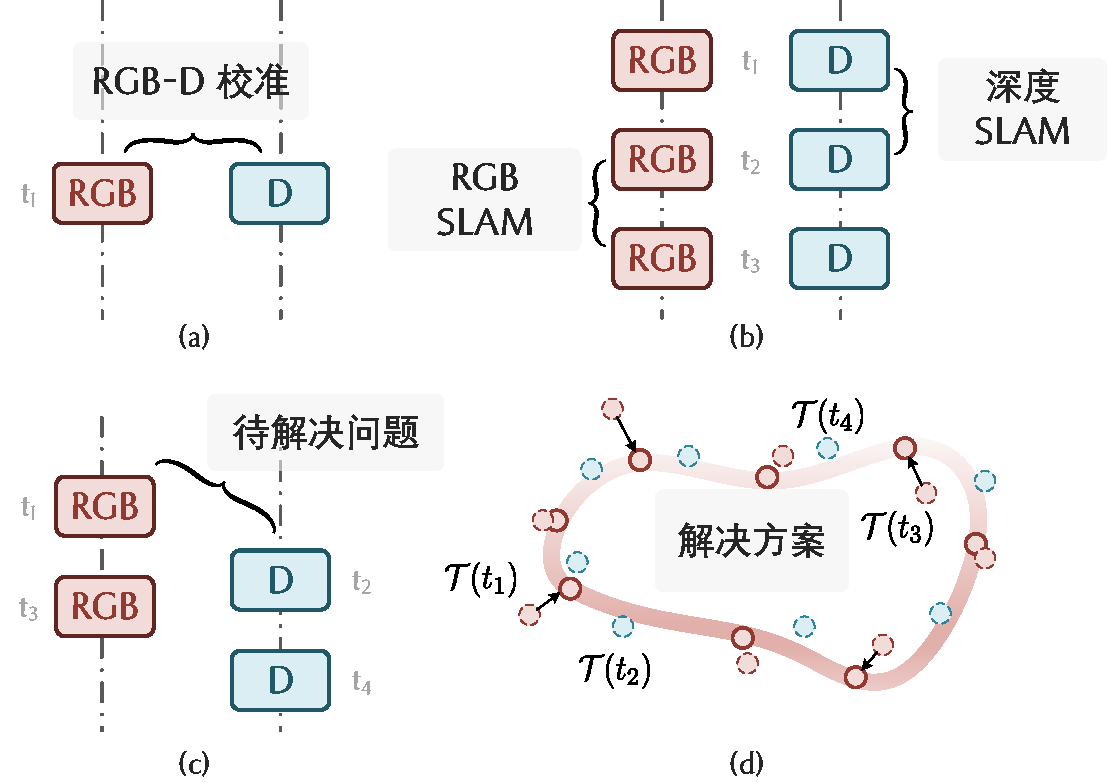
\includegraphics[width=0.8\textwidth]{undergraduate-thesis/images/time-pose function/teaser.pdf}
    \caption{本文感兴趣的问题与其他现有问题之间的比较的示意图。}
    \label{fig: time-pose function teaser}
\end{figure}

本文感兴趣的问题与图\ref{fig: time-pose function teaser}中广泛关注的其他现有问题进行比较:
\begin{enumerate}
    \item [(a)]RGB-D 校准方法\cite{jeong_self-calibrating_2021, bian_nope-nerf_2022}估计深度相机和 RGB 相机之间的变换关系,即内参数矩阵,此类方法通常使用点对点的配准方法来实现;
    \item [(b)] 给定连续获取的 RGB 或深度图,基于 RGB 的 SLAM\cite{campos_orb-slam3_2021, mur-artal_orb-slam_2015, engel_direct_2018, zhu_nicer-slam_2023}和基于深度的 SLAM \cite{niesner_real-time_2013, xu_multi-scale_2018}则估计相邻帧之间的转移矩阵 $\{T_{ij}\}$;
    \item [(c)] 本文感兴趣的问题则是通过从 RGB 序列的时间戳所对应的位姿序列中,学习其中隐含的轨迹先验来估计深度序列的相机轨迹$\{T_i^d\}$。
\end{enumerate}

\begin{figure}[t]
    \centering
    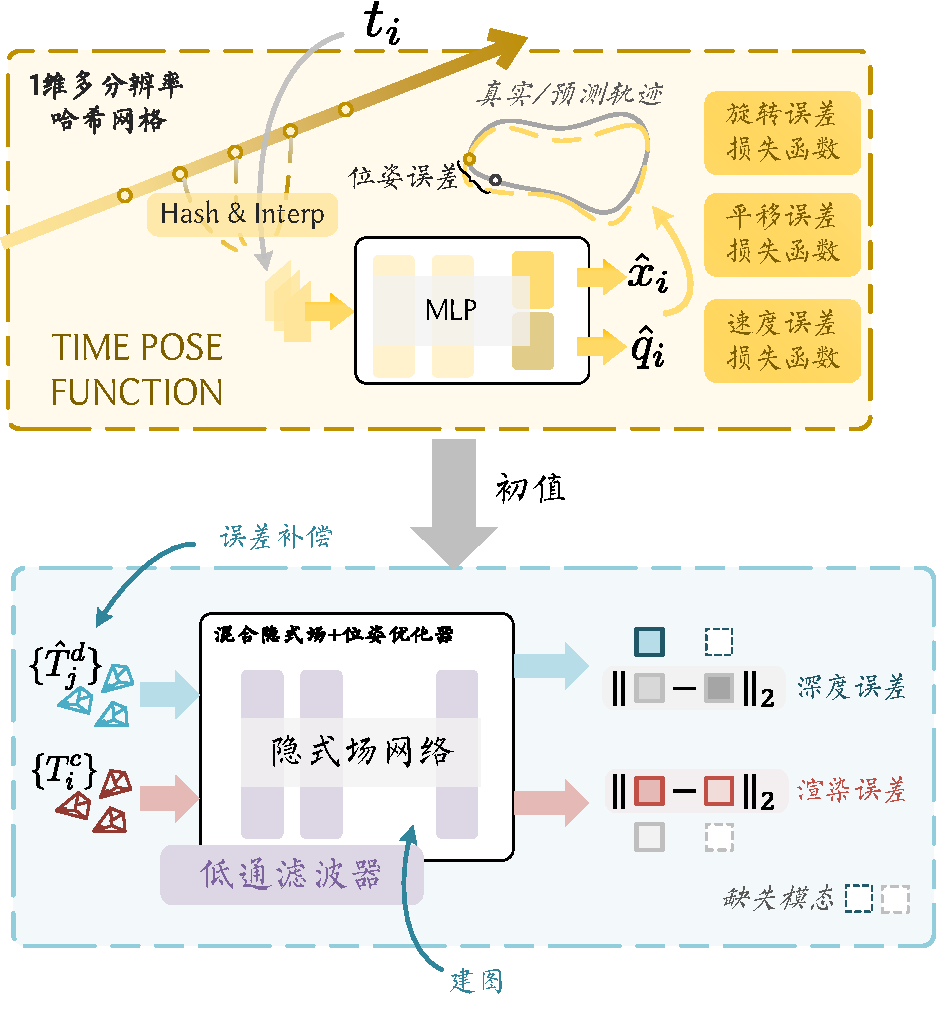
\includegraphics[width=0.8\textwidth]{undergraduate-thesis/images/time-pose function/main_export.pdf}
    \caption{系统概述图。本文的系统优化过程可以分为两个阶段。在第一阶段,TPF从 RGB 序列中时间和相机位姿之间的隐式函数关系中学习未知的深度相机位姿。在第二阶段,优化器同时训练具有深度监督的混合场景表示,并对估计的深度相机位姿进行精调。}
    \label{fig:time-pose function main figure}
\end{figure}

本节受到近期将神经辐射场与相机内外参数同时优化的方法\cite{yen-chen_inerf_2021, lin_barf_2021, bian_nope-nerf_2022}的启发,希望在时空不同步的RGB-D序列中同时恢复隐式场和相机位姿的方法。注意到这个问题存在一个自然的解决方案:
\begin{quote}
    将 RGB 和深度帧分别处理为在某些时间戳处具有\textbf{缺失模态}的相机捕获的帧。
\end{quote}

因此,以前的方法如 BARF\cite{lin_barf_2021} 可以很容易地扩展到这种情况,即在优化开始阶段为相机内外参任意赋予一个初始值,并在优化过程中通过反向传播算法不断调整。然而,这种基线方法未能在此问题中利用有用的特定领域先验,即RGB和深度相机实际上经过相同的连续运动轨迹。

为此,本文提出使用一种新型的时间-位姿隐函数(Time-Pose Function, TPF)对此先验进行建模,TPF将时间戳映射到六自由度相机位姿。就像神经符号距离场或辐射场中对具有 3D/5D 输入的函数进行逼近的方式一样, TPF逼近一个将 1D 时间戳作为输入并输出 SE(3) 流形\cite{sola_micro_2021}中的变换的函数。换句话说,这个TPF也是一个隐式场。本文将它与前文提到的混合隐式地图结合起来,形成如图\ref{fig:time-pose function main figure} 所示的级联架构。因此,在该框架下进行优化可以同时构建用于建图的城市规模混合隐式场,并校准 RGB-D 帧之间的不匹配问题。


\subsection{研究动机与问题描述}
问题。本文的目标是像 Mega-NeRF\cite{turki_mega-nerf_2022} 或 BungeeNeRF\cite{xiangli_bungeenerf_2022} 等先前工作中所做的那样,学习用于大规模场景表示的神经隐式场,这对于城市规划或机器人模拟等新兴应用至关重要。然而,这些先前的工作未能利用激光雷达等深度传感器捕获的几何信息。该问题现在已经收到了研究社区较大的关注\cite{deng_depth-supervised_2022,roessle_dense_2022},因为它可用于训练具有快速收敛性的无漂浮物 NeRF。为此,本文想解决在训练大规模隐式场时使用深度监督的问题。

\textbf{挑战:}
这个问题的基本挑战之一是异步 RGB-D 数据。然而目前为止,没有用于大型场景的易于访问的同步 RGB-D 传感器套件(如 RealSense 或 Kinect),并且根据时间戳简单地同步它们无法完全解决错位问题。本文没有将它们与昂贵的硬件严格同步,而是从算法的角度来看。这是一个新的自校准设置:在训练大规模 NeRF 的同时在线校准 RGB-D 相机变换。

\textbf{输入:} 在使用航空图像进行大规模场景建模的许多先前工作的基础上\cite{turki_mega-nerf_2022,xiangli_bungeenerf_2022},本文假设无人机捕获的输入 RGB-D 流:一组 RGB 相机图像$\{\mathcal{I}_i\}_{i=1}^{N_c}$和一组深度图$\{\mathcal{D}_i\}_{i=1}^{N_d}$。由于异步情况存在,这两个流在概念上如图\ref{fig: time-pose function teaser}-c所示,本文的目标是恢复它们之间的时空转换。鉴于本文的重点是相对变换,在不失一般性的情况下,将 RGB 或深度的位姿作为参考点都是可行的。为方便起见,本文假设彩色图像的相机位姿是通过 SfM 算法获得的,来预测深度图位姿。

\textbf{输出}:本文的最终目标是训练一个准确的神经隐式表示,在给定的视角$\mathbf{T}$下输出逼真的 RGB 图像$\hat{\mathcal{I}}$以及准确的深度图 $\hat{\mathcal{D}}$。同时,本文校准未知的深度相机位姿$\mathbf{T}_i^d$ 有助于引入深度监督以获得更好的场景表示。

\textbf{优化过程:}
为了利用隐式时间-位姿函数关系,本文建议使用基于回归的模型,该模型将 1D 时间戳作为输入并输出相应的 6-DOF 相机位姿。在实践中,本文使用 RGB 图像位姿来训练隐式时间位姿函数并在模型收敛后预测深度位姿。然而,时间关系本身可能无法为基于 NeRF 的神经渲染器提供足够的准确性,这需要像素级的准确性来构建逼真的场景图。因此,在第二阶段,本文在 NeRF 训练过程中同时优化最初预测的深度位姿,其中 RGB 和深度图像都用作监督信号。正如本文稍后在实验中所证明的那样,使用纯 RGB 监督优化神经隐式场足以实现照片般逼真的渲染;然而,学习到的场景几何可能无法满足真实世界的机器人应用需求。引入具有原始深度位姿对齐的深度传感监督甚至可能会损害准确性。为了利用无人机在同一轨迹上捕获 RGB 图像和深度图的先验,本文对 RGB-D 帧的时间戳$\{t_i\}_{i=1}^{N_c+N_d}$ 进行建模,并且相应的相机内在函数也取自EXIF 信息作为算法输入。

\begin{figure}[ht]
    \centering
    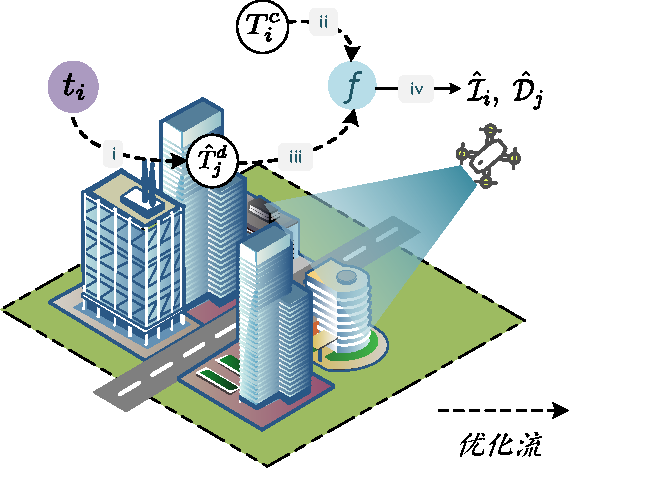
\includegraphics[width=0.6\textwidth]{undergraduate-thesis/images/time-pose function/Problem Formulation export.pdf}
    \caption{优化流程图}
    \label{fig:time-pose function optimization flow}
\end{figure}

\subsection{时间-位姿隐式轨迹函数 (TPF)}
在这一部分中,本文介绍了估计相机位姿的时间位姿函数 $\mathcal{T}$。本文将相机轨迹表示为隐式时间位姿函数,其输入是时间戳$t$,输出是 6-DoF 相机位姿。位姿输出由一个 3-D 平移向量 $x_i$ 和表示为四元数\cite{sola_micro_2021} $q_i$ 的 4-D 旋转向量组成。
\begin{equation}
    \mathcal{T}:\quad t_i\to\mathbf{T}_i=[x_i, q_i]
\end{equation}

\begin{figure}[ht]
    \centering
    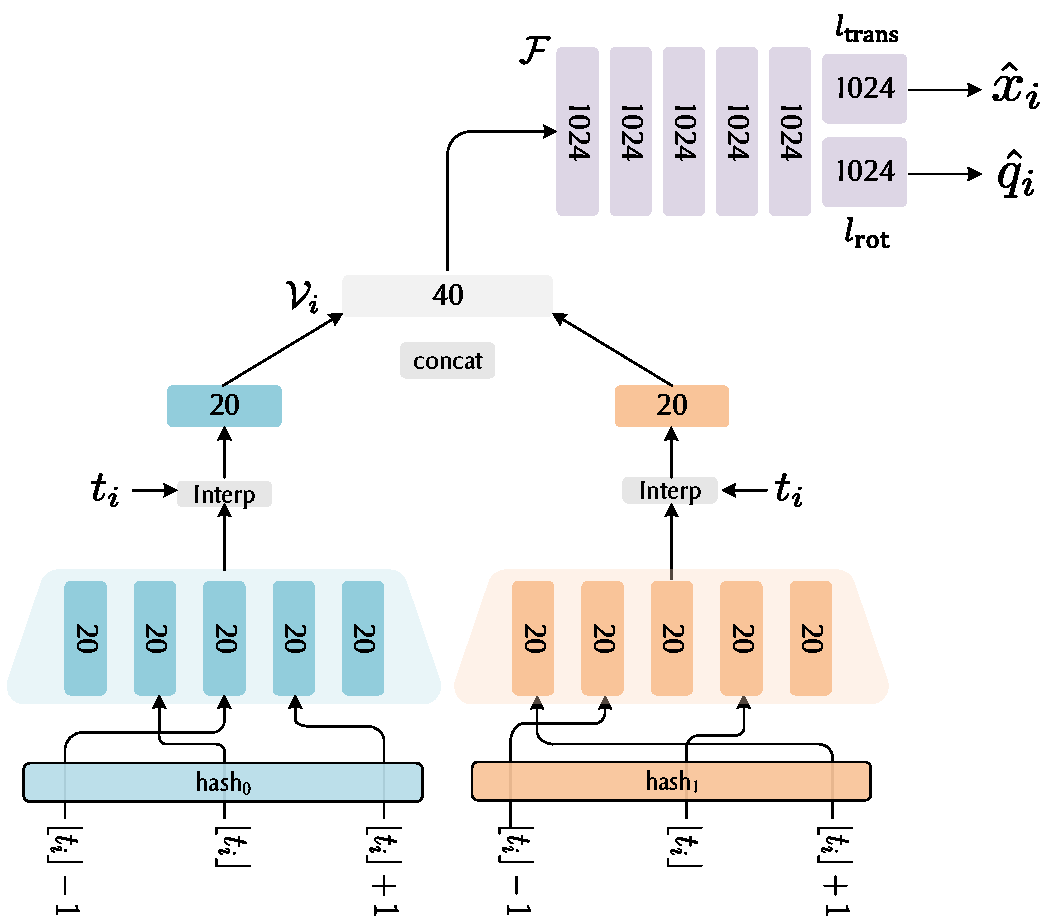
\includegraphics[width=\textwidth]{undergraduate-thesis/images/time-pose function/Hash.pdf}
    \caption{TPF的网络结构示意图。}
    \label{fig:time-pose function structure}
\end{figure}

\subsubsection{隐式TPF网络模型实现}

本文将TPF函数用一个一维多分辨率哈希网格 $\{G^{(l)}\}_L^{l=1}$ 近似,输出的参数会用一个浅层多层感知机解码器$\mathcal{F}_\Theta$解码。哈希网格由 $L$ 级独立的特征网格组成。当为所有时间戳范围内的任意时间戳 $t_i$ 查询相机位姿 $\mathbf{T}_i$ 时,本文从每个网格层采样哈希编码并对提取的编码后通过二次插值并连接在一起以获得特征向量 $\mathcal{V}_i$。获得内插特征向量后,使用共享 MLP 处理特征 $\mathcal{V}_i$,然后将其输出馈送到两个分离的全连接层,以分别预测输出平移 $x_i$ 和旋转 $q_i$ 向量。网络前传过程可以用以下等式表示:
\begin{align}
    \mathcal{V}_i&=\mathcal{F}_\Theta(\mathtt{concat}\{\mathtt{interp}(h(t_i;\pi_l), \mathcal{G}_\theta^l)\}^L_{l=1}),\\
    \hat{\mathbf{T}}_i &= [\hat{x}_i, \hat{q}_i] = l_{trans}(\mathcal{V}_i; \Theta_{trans}), l_{rot}(\mathcal{V}_i; \Theta_{rot}),
\end{align}
其中$\mathtt{interp}$表示插值算子,$h$是由$π_l$参数化的哈希函数,$l_{trans},l_{rot}$是两个全连接层,其中$\Theta_{trans},\Theta_{rot}$分别表示网络参数。

由于深度图和 RGB 图像都是由同一架无人机在同一飞行中收集的,因此除了两个传感器在飞机上的位置不同外,它们在时间和空间方面的轨迹几乎相同。因此,本文可以使用从 RGB 序列中学习到的隐式时间-位姿函数直接预测对应于深度序列时间戳的位姿,以及传感器位置之间已知的位姿变换 $\mathbf{T}_\text{sensor}$。


\subsection{优化TPF模型}
表示用于优化相机位姿的旋转的最常见选择是旋转矩阵\cite{yen-chen_inerf_2021}或 欧拉角。然而,由于它们与 SO(3) 的非同胚表示空间,它们在表示旋转时不是连续的\cite{kendall_posenet_2015}。本文选择使用单位四元数作为原始表示,因为任意 4-D 向量可以通过将它们归一化为单位长度轻松映射到合法的旋转。

为了优化时间-位姿函数,本文提出了以下目标函数:
\begin{equation}
    \mathcal{L} = \lambda_{trans}\mathcal{L}_{trans}+\lambda_{rot}\mathcal{L}_{rot}+\lambda_{speed}\mathcal{L}_{speed},
\end{equation}
其中,$\lambda_{trans}, \lambda_{rot}$会随着训练过程自动调整。本文将在后面介绍自适应权重。

\textbf{位移和旋转矢量的直接优化:}
本文通过评估估计相机位姿和地面实况相机位姿的均方误差 (MSE) 直接优化欧几里得空间中的平移和旋转向量:
\begin{align}
    \mathcal{L}_{trans} &= \text{MSE}(\{x_i\}, \{\hat{x}_i\})\\
    \mathcal{L}_{rot} &= \text{MSE}(\{q_i\}, \{\hat{q}_i\})
\end{align}

由于 $x$和 $q$ 的单位不同,因此比例因子 $\lambda_{trans}$ 和 $\lambda_{rot}$ 在平衡损失方面发挥了重要作用。为了防止平移和旋转在训练中相互产生负面影响并利用可能的相互促进作用,本文通过使用同方差不确定性 \cite{kendall_geometric_2017} 使加权因子可学习:\begin{equation}
    \mathcal{L}_{\sigma} = \mathcal{L}_{trans} \exp(−\hat{s}_{trans}) + \hat{s}_{trans} + \mathcal{L}_{rot} \exp( −\hat{s}_{rot}) + \hat{s}_{rot},
\end{equation}
其中 $\hat{s}$ 是可学习的,因此损失项会自动平衡。手动选择权重需要不断调整参数,但可以获得相似的性能。

\textbf{移动速度的梯度优化:}
观察到时间-位姿函数本质上是位移和角位移相对于时间的函数,本文可以使用平均线速度来监督网络输出相对于输入向量的梯度。这里平均速度是指从当前帧和相邻两个帧的地面真值相机位姿计算的平均值,而不是整个序列中的平均值。由于在无人机拍摄的场景中线速度变化较小,角速度变化相对较大,因此仅使用平均线速度来监督神经网络,而后者在本文的设置中没有受到监督:
\begin{equation}
    \mathcal{L}_{speed} = \text{MSE}(\{\frac{x_i-x_{i-1}}{t_i-t_{i-1}}\}, \{\hat{v}_i\})
\end{equation}

\subsection{后端优化与TPF误差补偿}
虽然时间-位姿函数为建图阶段提供了一个很好的深度相机位姿初始值,但在一些离群帧中仍然存在明显的错误。本文将描述如何同时执行映射和位姿优化,以补偿时间-位姿函数的误差。

对于地图表示,本文使用第\ref{chapter: omninerf}章所提出的混合隐式表达。在此基础指上,本文联合优化不准确的相机位姿和隐式映射:当优化场景表示参数 $\Theta_{Map}$ 时,估计的深度相机位姿 $\hat{\mathbf{T}}_i \in SE(3)$(其中 $t \in \mathbb{R}^3$, $q \in SO(3)$)将在流形上同时优化这些参数:
\begin{equation}
    \hat{\Theta}_{Map},\hat{\mathbf{T}} = \arg\min\mathcal{L}(\mathbf{T}, \Theta_{Map} | \mathbf{T}_0, \{\mathcal{I}_i\}, \{\mathcal{D}\}),
\end{equation}
其中 $\mathcal{L}$ 是目标函数,$\mathbf{T}_0$ 是时间-位姿函数的预测值。

为了补偿时间-位姿函数提取位姿的误差,本文通过应用一组可训练的位姿校正项进一步优化估计值。受 BARF\cite{lin_barf_2021} 的启发,在解决位置校准问题时,低频信号可以预测比高频信号更一致的位移,这很容易导致次优优化结果。传统 NeRF 渲染中的位置编码在高频细节方面显着改善了合成视图。使用可以削弱位置编码效果的低通滤波器将具有与平滑类似的效果。因此,在联合优化阶段中使用动态低通滤波器来帮助优化不准确的深度帧位姿。

\newpage
\section{雾天真实输入数据下的准确场景表示学习}
在上一节中介绍了如何配准不对齐的RGB-D序列,这一方法可以在真实场景中有效地融入深度信息。然而,在真实实验过程中同样发现,面对雾天、雨天等特殊天气情况时,由于深度传感器本身受影响较大,不能获得较为准确的传感器数据。然而另一方面,本文发现类似雾天这样的由于散射介质引起的图片退化可以从另一方面提供物体的深度信息。

因此在本节中,受最近对从特殊(例如,嘈杂或模糊)图像中学习隐式场的研究兴趣激增的启发,本文研究从模糊带雾图像中学习隐式场的问题。一个有趣的事实是,许多以前的方法侧重于避免不存在的漂浮物(通常指渲染出来的瑕疵),而本文希望通过建模\textbf{真正}的漂浮物来简介获得深度信息。本文首先证明,从模糊图像中学习的隐式场不能用于渲染可靠的深度,这与通过光衰减的雾度有关。为此,本文分析隐式场了学习到的体积密度值的分布,构建了一个加权函数,并证明了该函数可用于生成可信的深度图。同时,本文引入了协方差损失,用于消除颜色衰减和视点相关隐式之间固有的歧义。最后,本文通过编辑隐式场中的漂浮物密度来开发雾度处理管线。

\subsection{带雾场景分析}
新视图合成的最新进展利用神经辐射场来恢复复杂的场景几何和外观。由单个多层感知器参数化为场景坐标和相应场景量之间的映射函数,可以以自监督的方式从构成的多视图图像中学习隐式表示。优化的关键是体积渲染技术,该技术将像素值视为沿来自相机接收到的表面点的射线的辐照度的积分,从而保证光度误差反向传播到神经场。这种模式在大多数情况下都能很好地呈现照片级逼真度的新视图渲染结果。 
然而,大气中的悬浮颗粒,或者换句话说,漂浮物,会导致图像退化。这种现象在室外场景中非常常见(如雾天、霾天或烟雾等),他们主要由大气中漂浮物所产生的散射现象导致。这种模糊图像的退化导致相机接收到的辐照度减弱。这对从模糊图像中学习辐射场提出了挑战,因为在这种衰减的情况下,光度一致性不再成立。由于场景辐射和雾度之间固有的歧义,从模糊图像中监督场景的辐射场会导致嘈杂的几何形状和外观,如图所示。

\begin{figure}[ht]
    \centering
    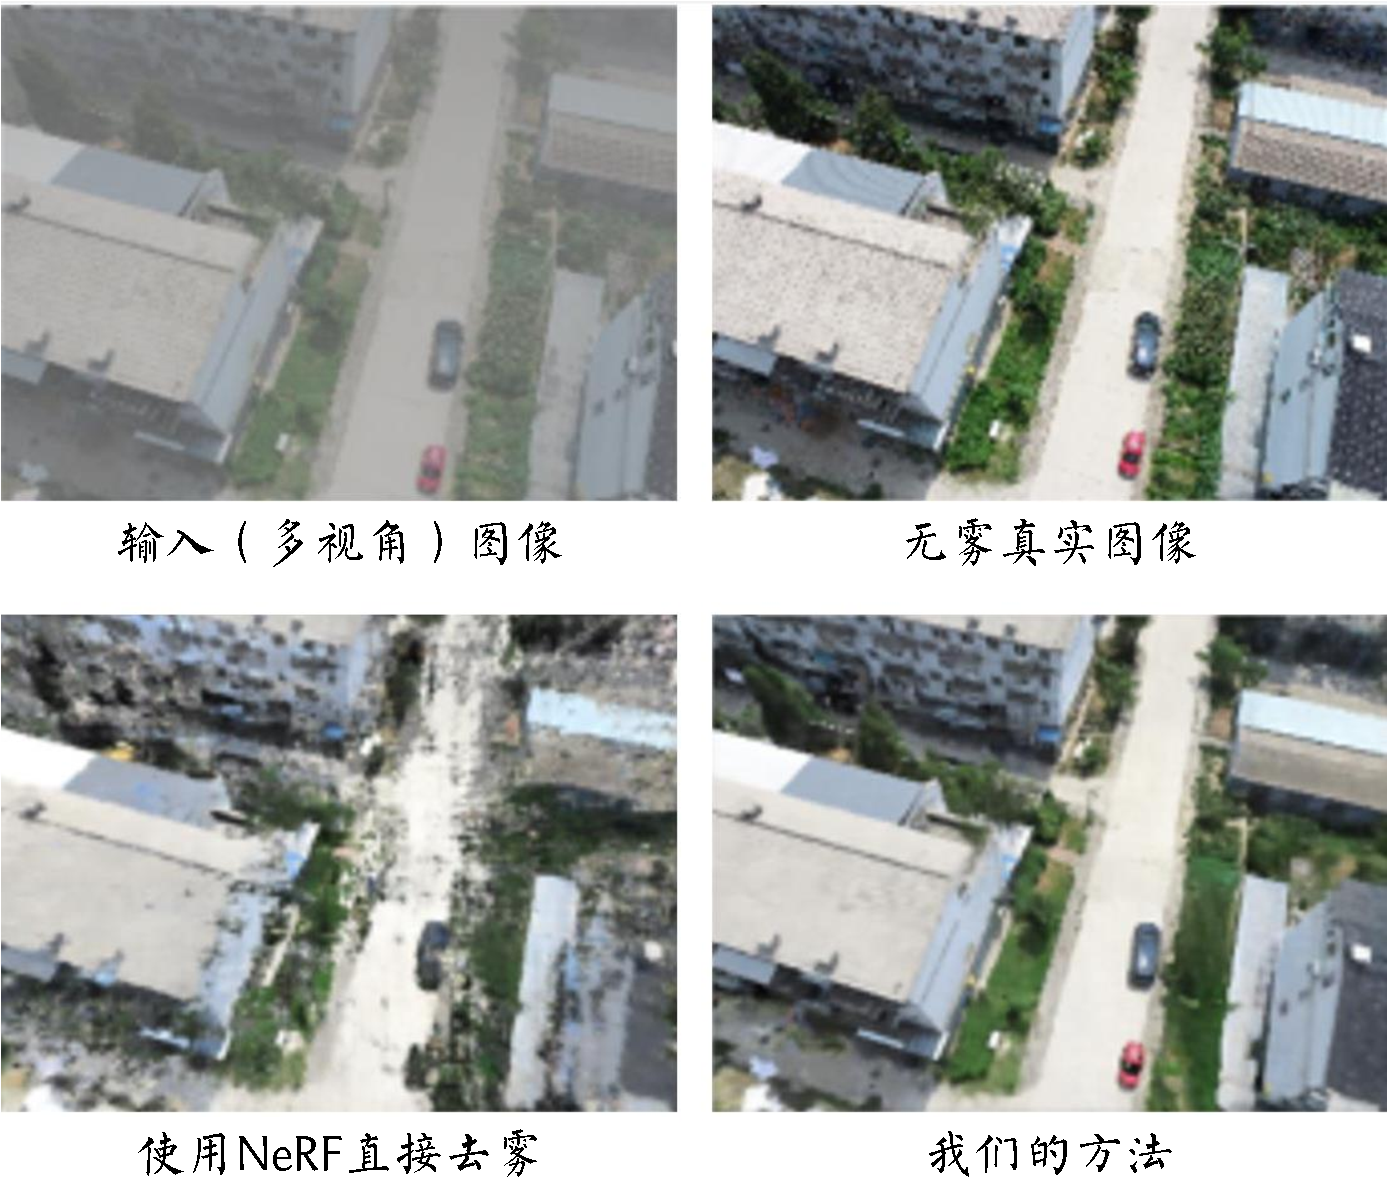
\includegraphics[width=0.8\textwidth]{undergraduate-thesis/images/dehazing-nerf/teaser.pdf}
    \caption{使用带雾图像进行多视角去雾。}
    \label{fig:dehazing-nerf teaser}
\end{figure}

通过分析辐射场内自然学习到的密度分布,本文首先深入探讨了漂浮物如何影响体积渲染过程的问题。从几何学上讲,漂浮物会导致地表前方的密度非零,因此渲染的深度图像会出现偏差,而从光度方面来看,由于传输依赖于深度,在不同距离观察朦胧场景可能会导致不同的结果即使场景辐射场与视图无关,视点之间的退化行为同样如此。这种有偏见的深度推理和模棱两可的视图依赖性导致辐射场的学习难以处理。为了解决这些问题,本文提出了一种改进的深度图细化平均权重。就视图依赖性歧义而言,本文引入了一个基于协方差的正则化项,以减小辐射和雾霾引起的辐照度衰减之间的强耦合。这些方式保证了无雾场景表示的准确恢复以及漂浮物的浓度控制。

\begin{figure}[ht]
    \centering
    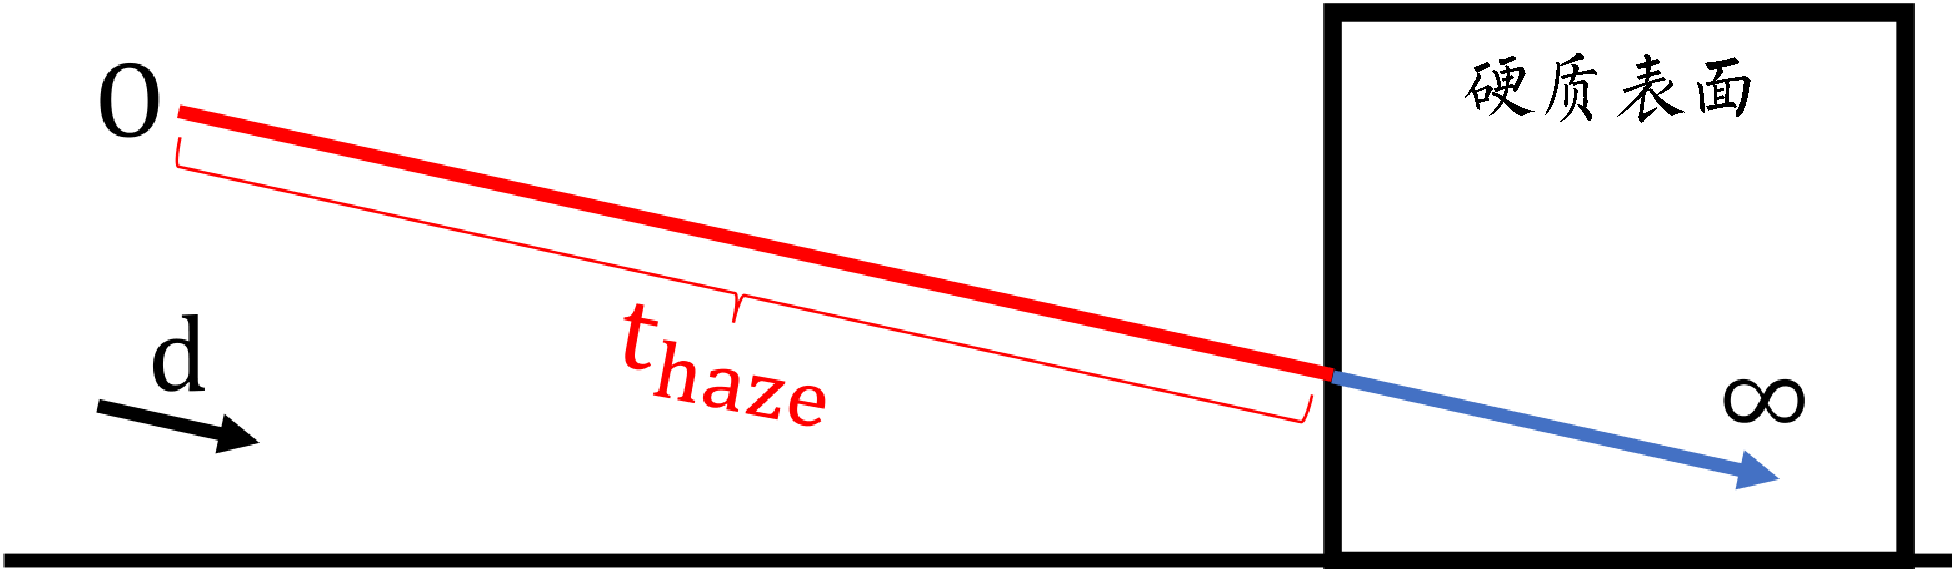
\includegraphics[width=\textwidth]{undergraduate-thesis/images/dehazing-nerf/t-haze.pdf}
    \caption{射线经过带雾空气和硬质表面的示意图。}
    \label{fig:dehazing-nerf t-haze decomposition}
\end{figure}

\subsection{散射介质的理论模型分析}
为什么使用 NeRF 去雾是一个自然合理的选择?本文首先证明体积渲染公式可以重新分解为DCP\cite{kaiming_he_single_2009}中广泛使用的薄雾方程。在有雾的场景中,公式可以分为两部分,分别对雾霾(图\ref{fig:dehazing-nerf t-haze decomposition}中的红色部分)和硬质结构(图\ref{fig:dehazing-nerf t-haze decomposition}中的蓝色部分)进行积分。假设$t_{haze}$(在图\ref{fig:dehazing-nerf t-haze decomposition}中)表示相机原点与采样光线与硬质结构的交点之间的距离,即雾度的深度。通过从硬质结构部分移出常数项 $T_{haze} = T(t_{haze})$,体渲染公式可以进一步解释为:
\begin{align}
    \textbf{c}(\textbf{r}) &= \int_{t_n}^{t_{haze}}T(t)\sigma(t)c(t)\text{d}t + T_{haze}\int_{t_{haze}}^{t_f}T'(t)\sigma(t)c(t)\text{d}t\\
    \textbf{d}(\textbf{r}) &= \int_{t_n}^{t_{haze}}T(t)\sigma(t)t\text{d}t + T_{haze}\int_{t_{haze}}^{t_f}T'(t)\sigma(t)t\text{d}t,
\end{align}
其中$T'(t)=\exp(-\int_{t_{haze}}^{t}\sigma(\tau)\text{d}\tau)=T(t)/T_{t_{haze}}$。

这样的分解形式正好可以与DCP中常见的带雾图像形成公式相对应:
\begin{equation}
    \mathbf{I}= \textcolor{red}{\mathbf{A} (1-\mathbf{T})} + \textcolor{blue}{\mathbf{J} \mathbf{T}}
\end{equation}
其中$\mathbf{T}=\mathbf{e}^{-\beta \cdot t_\text{haze}}$.

先看蓝色部分。通过将图\ref{fig:dehazing-nerf t-haze decomposition}中红色区域的密度视为零,无雾图像 $\mathbf{J}$ 可以对应于$\int_{t_{haze}}^{t_f}T'(t)\sigma(t)c(t)\text{d}t$。累计透光度 $\mathbf{T}$ 对应于 ${T_{haze}}$。然后看红色部分,在均匀雾度的情况下, $σ(t)c(t)$ 变为常数,可以从等式的第一项移出,即:
\begin{align*}
    \textcolor{red}{\int_{t_n}^{{t}_\text{haze}}\mathbf{T}(t){{\sigma}}(t){\mathbf{c}}(t)\mathbf{d}t} &= \int_{t_n}^{t_\text{haze}} \text{exp}(-\int_{t_n}^t {\sigma}\mathbf{d}\tau) {\sigma}{\mathbf{c}}\mathbf{d}t \\
    &=\int_{t_n}^{t_\text{haze}} \text{exp}(-{\sigma}t) {\sigma}{\mathbf{c}}\mathbf{d}t \\
    &={\sigma}{\mathbf{c}}\int_{t_n}^{t_\text{haze}} \text{exp}(-{\sigma}t) \mathbf{d}t \\
    &={\sigma}{\mathbf{c}}(-\frac{1}{{\sigma}}\text{exp}(-{\sigma}t))\big|_{t_n}^{t_\text{haze}} \\
    &=\textcolor{red}{\mathbf{A}(1-\mathbf{T})}
\end{align*}

根据上述方程式的对应关系,可以很自然地使用NeRF来达到多视角去雾或进行雾浓度控制的目的。根据等式将场景划分为雾霾和固体结构。通过只修改雾霾区域的属性,就可以达到去雾和雾霾操纵的目的。然而,恢复方程中变量的准确值并非易事,即像素方向的雾度深度 $t_{haze}$ 和场景的隐式表示。主要原因如下:
\begin{itemize}
    \item \textbf{偏差的深度渲染}。估计 $t_{haze}$ 的一个直接想法是使用标准深度渲染函数对其进行近似。然而,注意到雾霾或漂浮物的体积密度不为零,因此方程式中雾霾的积分权重也不为零。距离小于 $t_{haze}$ 的非零权重会使方程式中的加权积分产生偏差,使渲染的深度通常小于实际雾度深度$t_{haze}$。
    
    \textbf{解决方案:}为了解决这种偏差,本文调整了深度渲染函数,通过将其整体权重更改为定制的替代函数 $w_D$(参见下文)。然后使用修改后的权重重新渲染像素深度图。这个新的权重函数是根据三个必要条件设计而成的,可以确保渲染的深度图非常接近实际的深度图。
    \item \textbf{二义性问题}。此外,要学习准确的场景隐式表示,解决歧义问题很重要。原始 NeRF 方法仅使用光度误差来优化网络,然而颜色可以通过几何和辐射的不同组合来解释(即形状-辐射二义性\cite{zhang_nerf_2020})。例如,在图 \ref{fig:dehazing-nerf taxonomy}中,渲染图像中的边缘可能会随着雾度密度的变化而出现或消失,并且不同观察方向的色差可能是由光衰减和视图相关效应引起的。
    \textbf{解决方案:}本文通过使用距离和 RGB 值之间的相关性对其进行建模来解决多视图下朦胧场景的模糊性问题。本文在这两个变量之间添加协方差损失。这种损失有助于稳定训练过程并减少显色方面的歧义。
\end{itemize}

\begin{figure}[ht]
    \centering
    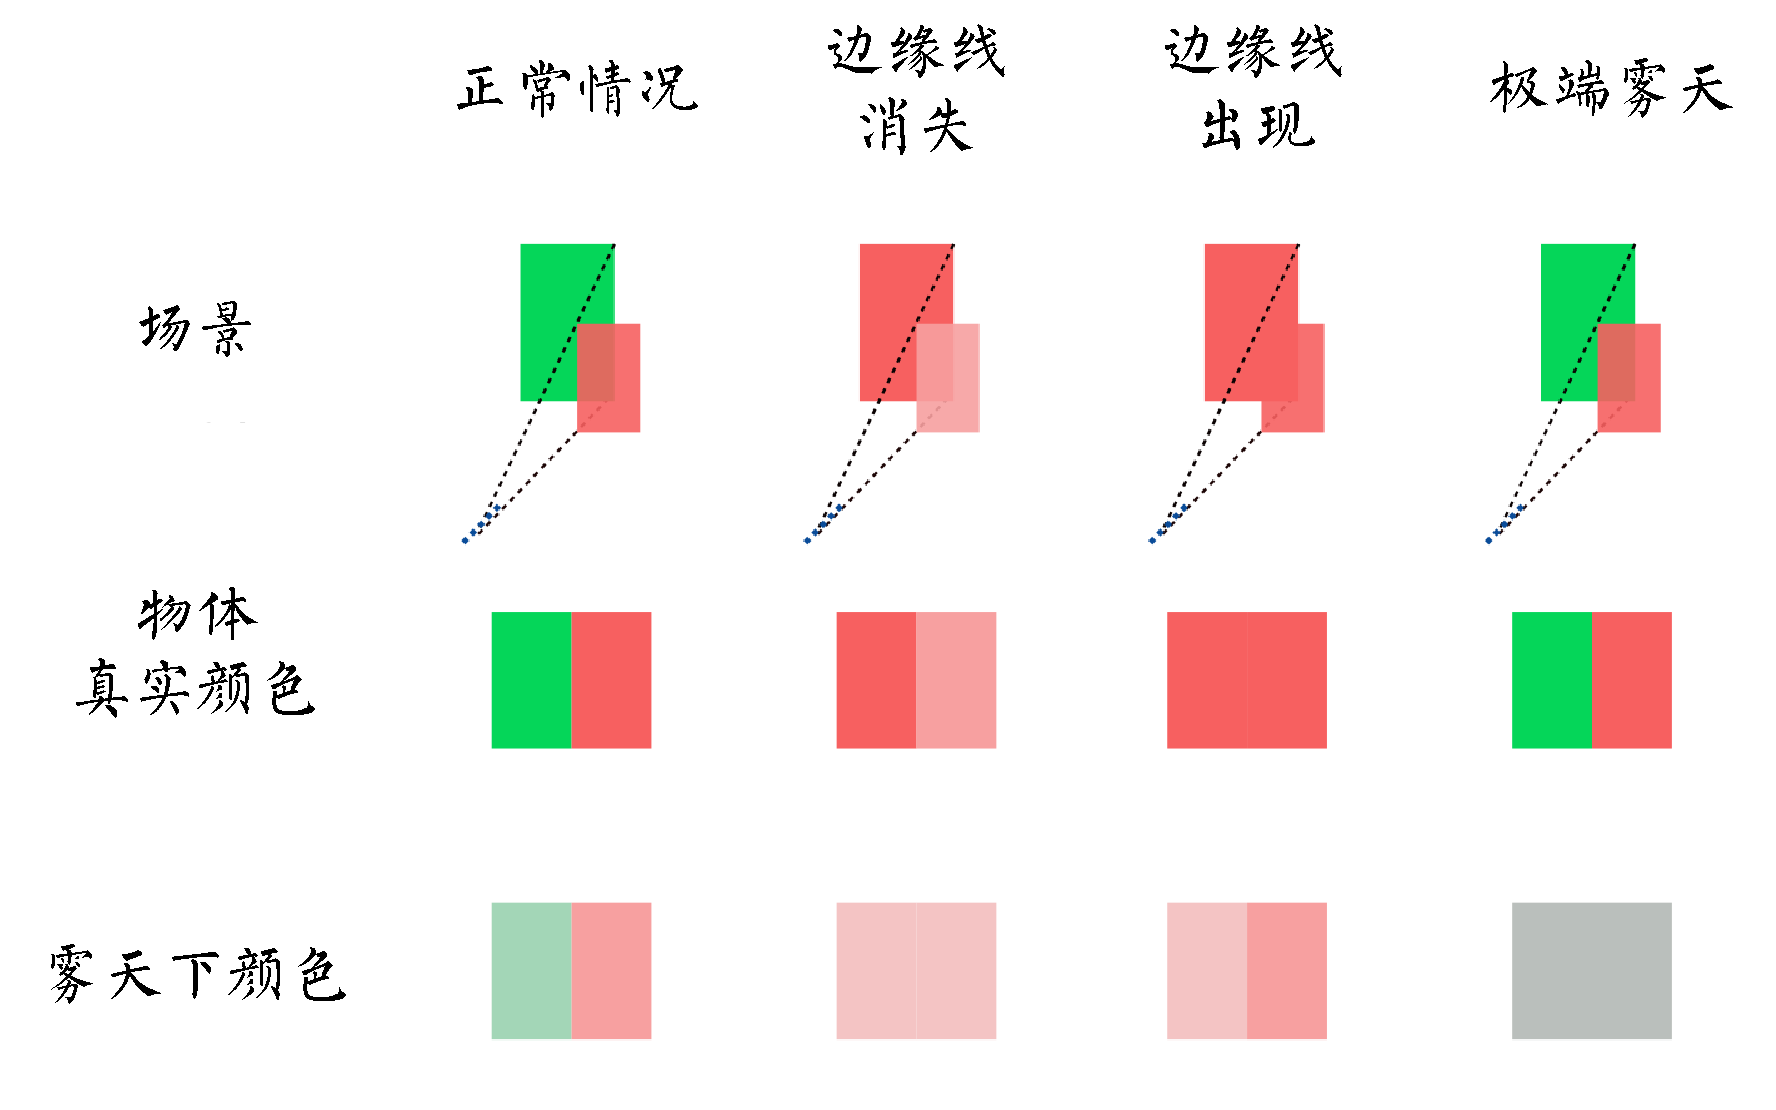
\includegraphics[width=\textwidth]{undergraduate-thesis/images/dehazing-nerf/taxonomy.pdf}
    \caption{不同场景在雾天情况下的观察颜色和实际颜色情况的分类图。}
    \label{fig:dehazing-nerf taxonomy}
\end{figure}

\subsection{建立忽略散射效应的深度权重函数}
在清晰、无雾的图像上训练的 NeRF 网络的体积密度输出遵循一种模式,即在表面位置附近取大值,在相机原点和表面之间取接近于零的值。这种模式在物理上是合理的,并已被许多作品使用,例如 NeuS \cite{wang_neus_2021},NeuralRGb-D\cite{azinovic_neural_2022} 和深度监督 NeRF\cite{deng_depth-supervised_2022}。这种模式允许方程式中的 NeRF 渲染权重 $w_{RGB}$, 在除表面附近以外的所有位置都取接近于零的值,渲染深度 $D$ 以准确地近似表面深度。

然而,这种模式不再适用于雾天的场景。空气中悬浮粒子的体积密度不为零,可以取任意值。如果仍然使用普通体渲染公式,雾霾位置的权重会明显大于清晰场景中的权重,从而使渲染深度产生偏差。因此,需要针对有雾场景的深度权重设计一个深度权重函数。这对于确保准确的深度估计和高质量的去雾结果是必要的。通过将表面深度定义为:
\begin{equation}
    \hat{D} =\int_0^\infty w_D(t)\cdot t\text{d}t,
\end{equation}
本文利用固体结构的密度明显大于雾度的特性,并使用新的深度权重函数 $w_D$ 应遵循的三个条件:
\begin{enumerate}
    \item \textbf{散射不敏感性}: 给定两个深度值 $t_1$ 和 $t_2$,如果 $\mathbf{thresh} > \sigma (t_1) >> \sigma (t_2)$,则 $ \mathbf{w}_\text{D}(t_1) >> \mathbf{w}_\text{D}(t_2) > 0$ 且 $\frac{\mathbf{w}_\text{D}(t_1)}{\mathbf{w}_\text{D}(t_2)} >> \frac{\sigma (t_1)}{\sigma (t_2)}$。
% 1) \textbf{Haze insensitivity}: $ \mathbf{w}_\text{D}(t_1) >> \mathbf{w}_\text{D}(t_2) $ if $ \mathbf{thresh} > \sigma (t_1) >> \sigma (t_2)$.
空气中漂浮物质的体积密度明显小于固体表面的体积密度。因此,高体积密度的位置更有可能是表面点。因此,在体积密度更高的位置分配一个压倒性的更大权重非常重要。

这个条件只需要在可能出现雾的区域中满足,因此本文设置一个阈值 $\mathbf{thresh}$,它是可能的雾体积密度的上限。值得注意的是,$\mathbf{thresh}$ 不需要是最小的上界,因为太大的值不会直接破坏雾和固体结构之间的区别。

漂浮物质的体积密度明显小于固体表面的体积密度。在某种程度上,体积密度越高,更有可能出现在表面点上。因此,具有更高体积密度的位置应该具有压倒性的更大权重。此外,在多个表面互相覆盖的情况下,NeRF 可能会为被覆盖表面输出更高的体积密度。但是,覆盖表面的体积密度足够大,使其成为不透明。为了避免关注覆盖表面,设置了一个软阈值。如果两个点的体积密度都超过阈值,则它们都被视为不透明,权重的比较关系不需要保持。

\item \textbf{遮挡感知性:} 给定两个深度值 $t_1$ 和 $t_2$,其中 $\mathbf{w}_\text{RGB}(t_1) >> \mathbf{w}_\text{RGB}(t_2)$,则 $ \mathbf{w}_\text{D}(t_1) >> \mathbf{w}_\text{D}(t_2)$。
由于 NeRF~\cite{mildenhall_nerf_2020} 在其权重计算 $\mathbf{w}_\text{RGB}$ 中自然地编码了遮挡,因此新的权重输出不应破坏表面之间的遮挡关系。


\item \textbf{归一化:} $ \int_0^{+\infty} \mathbf{w}_\text{D} \cdot {d}t = 1 $。
\end{enumerate}

本文深度权重函数的最终条件是一个归一化条件,它强制所有位置的权重总和为$1$。这个条件保证整个积分方程符合加权平均的形式。
\begin{figure}[ht]
    \centering
    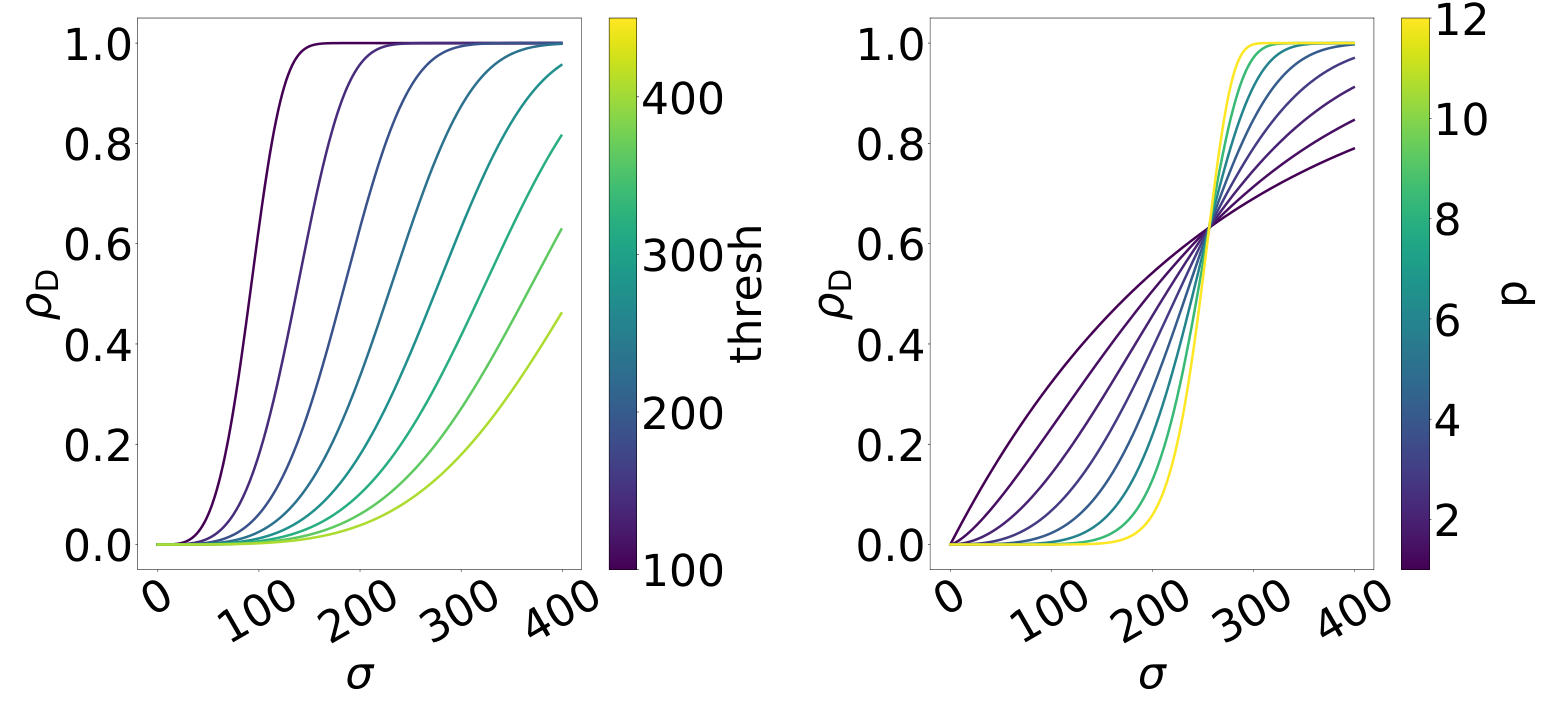
\includegraphics[width=\textwidth]{undergraduate-thesis/images/dehazing-nerf/function-family.png}
    \caption{不同阈值和 $p$ 值下函数 $w_\text{D}$ 的可视化示例:}
    \label{fig:dehazing-nerf function-family}
\end{figure}
有许多解决方案可以满足本文概述的三个条件。这里,本文提供一个满足第一个条件的 $\rho_\text{D}$ 函数的示例:
\begin{equation}
    \rho_\text{D}(t) = 1 - \exp\left\{-\left[\frac{\sigma(t)}{\mathbf{thresh}}\right]^p\right\}.
\end{equation}

本文构造的 $\rho_\text{D}$ 函数在 $\sigma << \mathbf{thresh}$ 时近似于幂函数 $\mathbf{const}\cdot \sigma^p$,并在 $\sigma > \mathbf{thresh}$ 时逐渐收敛到 1。这里引入了两个因素:$p$ 和 $\mathbf{thresh}$。图 \ref{fig:dehazing-nerf function-family} 展示了不同设置下的 $\sigma-\rho_\text{D}$ 曲线。$\mathbf{thresh}$ 代表可能的雾化位置体积密度和可行的实体位置体积密度之间的边界。$p$ 表示对 $\mathbf{thresh}$ 的置信水平;$p$ 越高,雾化和实体结构之间的分离就越清晰。

本文修改了 $\rho_\text{D}$ 函数以满足第二和第三个条件,得到:

\begin{equation}
w_\text{D}(t) = \frac{\rho_\text{D}(t) \mathbf{w}_\text{RGB}(t)\text{d}t}{\int_0^\infty \rho_\text{D}(t) \mathbf{w}_\text{RGB}(t)\text{d}t}.
\end{equation}

因此,为了满足遮挡感知的条件,本文将函数 $\rho_\text{D}$ 乘以 NeRF 渲染权重函数 $w_\text{RGB}$。然后,为了满足第三个条件,本文通过将函数 $w_\text{D}$ 除以 $\rho_\text{D}(t) w_\text{RGB}(t)\text{d}t$ 在 0 到无穷大范围内的积分来进行归一化。这个归一化条件保证了积分方程遵循加权平均的形式。

通过构造满足所有三个条件的深度权重函数,本文能够精确地估计雾化场景中的深度,并实现高质量的去雾结果。

\subsection{处理视角相关-颜色二义性}
传统的神经辐射表征方法~\cite{mildenhall_nerf_2020}使用一个5D函数来编码点辐射,其输入为3D点坐标和视角方向,以建模Lambertian效应(如高光)。然而,在NeRF中,RGB辐射与视角方向之间的关系受到的限制较少。这在训练雾化场景时会导致严重的歧义。

\subsubsection{为什么NeRF中的视角依赖性会导致在学习雾天场景表示时出现歧义}

在雾化场景中,由于高光和雾/漂浮物的复合效应,同一3D点的颜色观测会因不同的视角而异。然而,NeRF网络中的限制并未提供一个基础来分离混合效应。网络会误解由于受到雾化颜色衰减而导致的颜色变化,并返回具有视角依赖性的辐射结果,即使实际上场景中的所有点都具有视角无关的辐射。

一种简单直接的方法是利用Lambertian效应在雾天中被抑制的先验知识,显式地消除辐射场中的视角依赖性。在大多数情况下,这种方法确实是有用的。但它只是一种规避问题的方式。它无法表示在极具Lambertian效应的极度雾化场景和几乎没有雾化衰减效应的极度晴朗场景之间的中间情况。
本文在这里提出了一种距离和辐射值之间的协方差损失,这在理论和实践上都解决了这个问题。

\begin{figure}[ht]
    \centering
    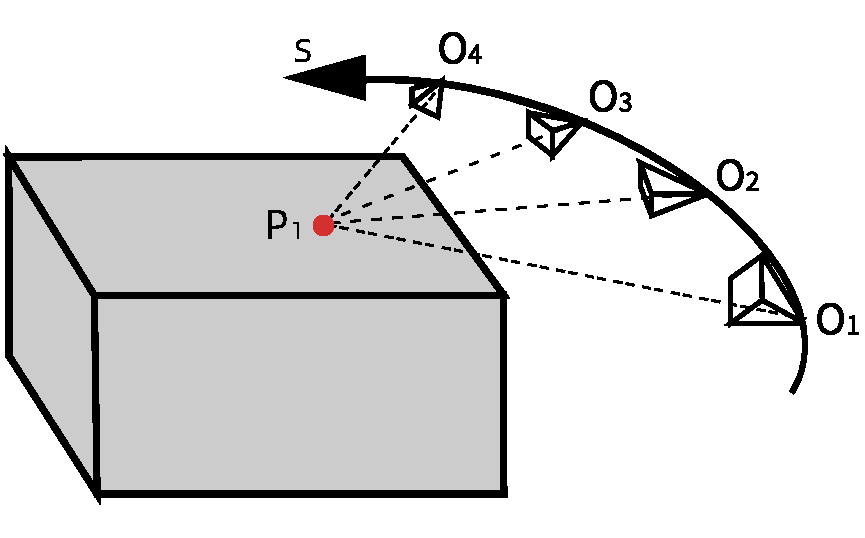
\includegraphics[width=0.6\textwidth]{undergraduate-thesis/images/dehazing-nerf/s-multivalues_example.pdf}
    \caption{相机位姿轨迹和弧长参数化的示例。本文假设相机沿着曲线移动,变量$s$表示当前相机位置和曲线原始位置之间的弧长距离。}
    \label{fig:dehazing-nerf s-multivalues_example}
\end{figure}

\subsubsection{深度-辐射协方差损失函数}
在本部分中,本文假设摄像机的运动遵循一个隐式轨迹曲线,如图\ref{fig:dehazing-nerf s-multivalues_example}所示。尽管图\ref{fig:dehazing-nerf s-multivalues_example}展示了一个简单而平滑的轨迹,但以下结论对于任意复杂的轨迹也成立。 对于固定的采样点 $\mathbf{P}_1$,从不同相机位置 $\mathbf{O}_i$ 的多条光线经过它。可以使用 $\mathbf{P}_1$、方向 $\mathbf{d}_i$ 和雾距离 ${t}_\text{haze\: i}$ 来反向表示 $\mathbf{O}_i$ 的坐标:
\begin{equation}
    \mathbf{O}_i = \mathbf{P}_1 - {t}_\text{haze\: i} \cdot \mathbf{d}_i。
\end{equation}

渲染方程中的项是$\mathbf{O}_i$和$\mathbf{d}_i$的函数,因此它们现在可以用$\mathbf{d}_i$、$\mathbf{P}_1$和${t}_\text{haze\: i}$来表示。本文将这些项列举如下:

由于各种光效应引起的悬浮粒子辐射为:
\begin{equation}
    \mathbf{C_\text{haze}}(\mathbf{d}_i, \mathbf{P}_1, {t}_\text{haze\: i}) = \int_0^{{t}_\text{haze\: i}} \mathbf{T}(t)\hat{\sigma}(t)\hat{\mathbf{c}}(t)\mathbf{d}t,
\end{equation}

悬浮粒子引起的衰减因子为:
\begin{equation}
    \mathbf{T_\text{haze}}(\mathbf{d}_i, \mathbf{P}_1, {t}_\text{haze\: i}) = \mathbf{T}({t}_\text{haze}),
\end{equation}

在被悬浮粒子衰减之前从实体结构发出的辐射为:
\begin{equation}
    \mathbf{C_\text{struct}}(\mathbf{d}_i, \mathbf{P}_1, {t}_\text{haze\: i}) = \int_{{t}_\text{haze}\: i}^{\infty}\mathbf{T}'(t)\hat{\sigma}(t)t\mathbf{d}t,
\end{equation}

相机捕获的最终RGB值为:
\begin{equation}
\begin{split}
    &\mathbf{C_\text{final}}(\mathbf{d}_i, \mathbf{P}_1, {t}_\text{haze\: i}) = \mathbf{C}(\mathbf{O}_i, \mathbf{d}_i) \\
    = &\mathbf{C_\text{haze} + T_{haze} \cdot C_\text{struct}}. \label{eq:ObservedColor}
\end{split}
\end{equation}
\newcommand{\slfrac}[2]{\left.#1\middle/#2\right.}

将体积密度项$\hat{\sigma}(t) = \sigma(\mathbf{O} + t\mathbf{d})$和RGB颜色项$\hat{\mathbf{c}}(t) = \mathbf{c}(\mathbf{O} + t\mathbf{d})$展开后,可以证明在几乎所有有雾的场景中,对于所有相机起点,偏导数$\slfrac{\partial}{\partial {t}_\text{haze: i}}(\mathbf{C_\text{haze}})$和$\slfrac{\partial}{\partial {t}_\text{haze: i}}(\mathbf{T_\text{haze}})$均为非零值。相反,$\slfrac{\partial}{\partial {t}_\text{haze: i}}(\mathbf{C_\text{struct}})=0$始终成立。

如图\ref{fig:dehazing-nerf s-multivalues_example}所示,摄像机起点运动曲线可以使用弧长参数化$\mathbf{s}$进行参数化。摄像机起点的坐标可以表示为$\mathbf{O}_i = \mathbf{O}(\mathbf{s}_i)$,其中$\mathbf{s}_i$是隐式轨迹曲线上的样本点。光线方向和雾深度也可以表示为:
\begin{equation}
    \mathbf{d}_i = \mathbf{Normalize}(\mathbf{O}(\mathbf{s}_i) - \mathbf{P}_1), \label{eq:direction}
\end{equation}
\begin{equation}
    \mathbf{\tilde{t}_\text{haze}}(\mathbf{s}, \mathbf{P}_1) = t_\text{haze\: i} = \left\|\mathbf{O}(\mathbf{s}_i) - \mathbf{P}_1\right\|_2.
\end{equation}

\begin{figure}[ht]
    \centering
    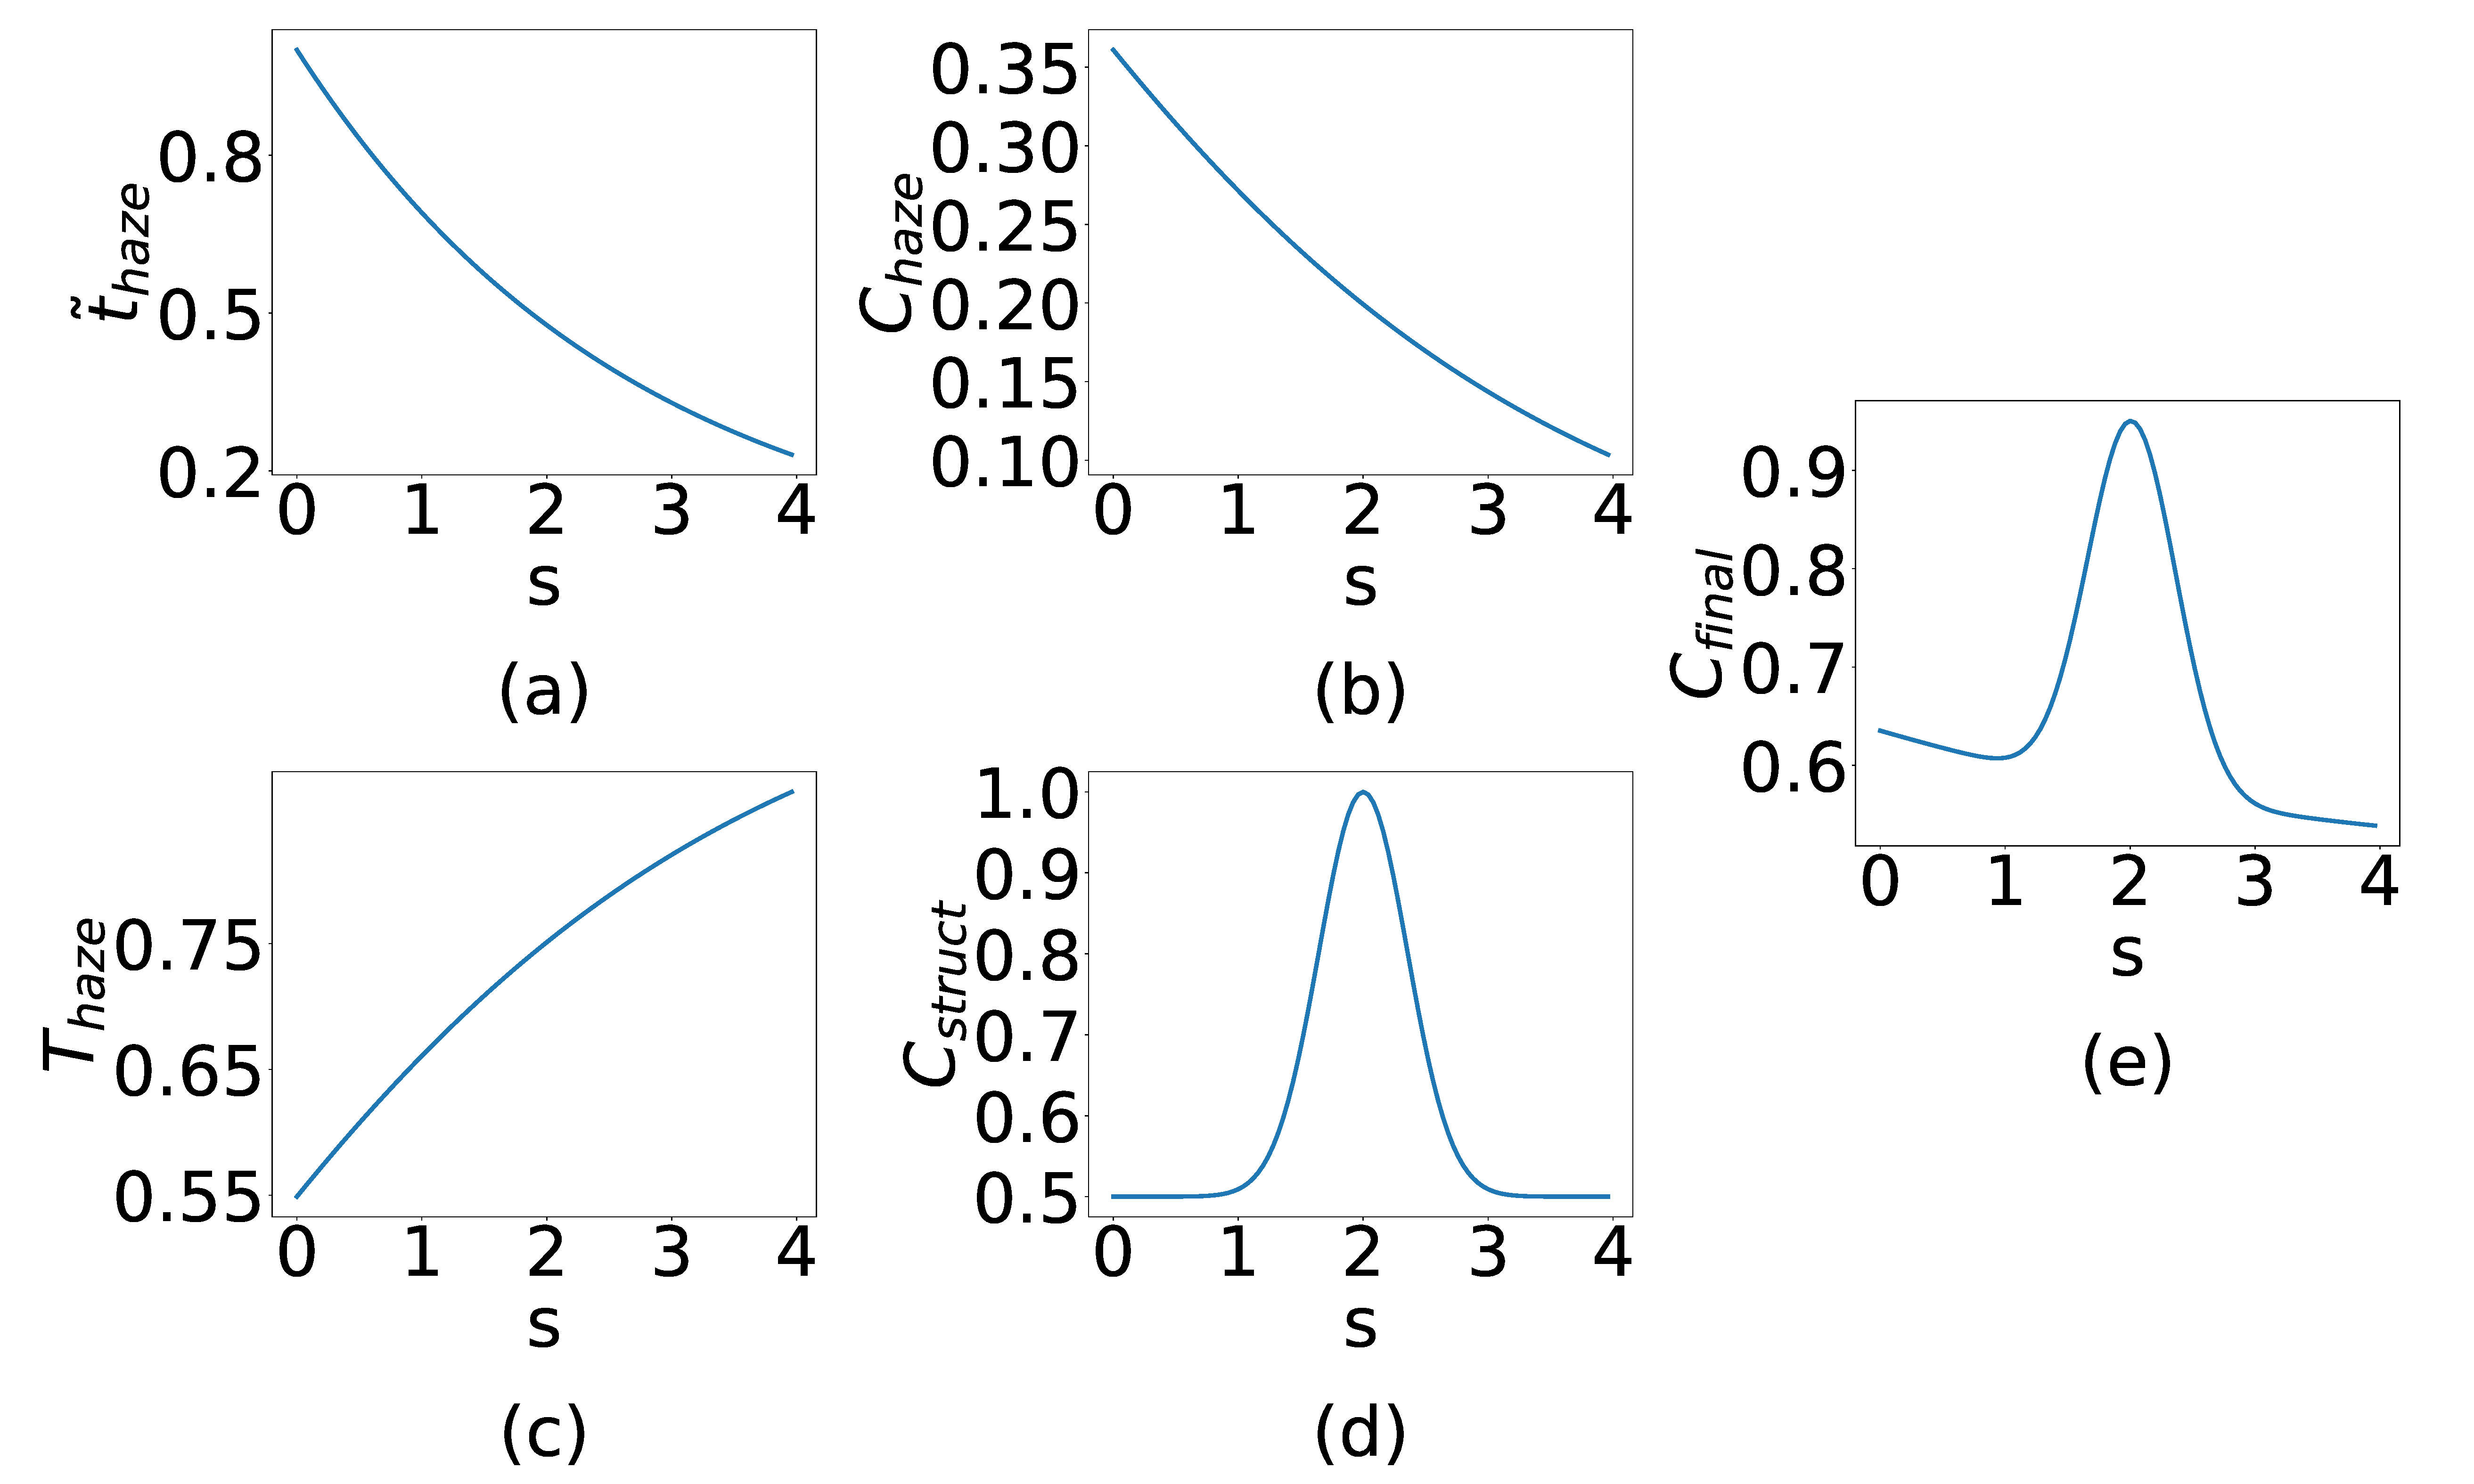
\includegraphics[width=\textwidth]{undergraduate-thesis/images/dehazing-nerf/s-multivalues_relation.pdf}
    \caption{根据图\ref{fig:dehazing-nerf s-multivalues_example}描述的场景,本文演示了随着摄像机沿曲线移动,摄像机与表面之间的距离减小,从而散射悬浮颗粒所导致的颜色(雾颜色)也会减小。射线与表面相交点处的透射率增加,因为漂浮物占据的自由空间减少了。但是,表面辐射独立于摄像机运动而改变(可能是由于镜面效应)。}
    \label{fig:dehazing-nerf view-dependency_relation}
\end{figure}

通过将样本点的所有可观测变量写成弧长参数的函数,本文可以在二维可视化展示这些函数随$s$的变化,如图\ref{fig:dehazing-nerf view-dependency_relation}所示。对于固定在对象表面上的点$\mathbf{P}_1$,这些图清晰地显示了$\mathbf{C_\text{haze}}$和$\mathbf{T_\text{haze}}$与$\mathbf{\tilde{t}_\text{haze}}$相关,而$\mathbf{C_\text{struct}}$则不相关。此外,这些图说明了这些变量如何影响$\mathbf{C_\text{final}}$。换句话说,在方程\ref{eq:ObservedColor}中,$\mathbf{C_\text{struct}}$是唯一与${t}_\text{haze: i}$无关的项。

值得注意的是,NeRF使用的光度损失仅与$\mathbf{C_\text{final}}$有关。因此,通过消除深度对$\mathbf{C_\text{struct}}$值的影响,训练过程可以恢复为无歧义的过程。对于表面点$\mathbf{P}_1$,$\mathbf{C_\text{struct}}$值近似于该点的辐射值$\mathbf{c}(\mathbf{P}_1, \mathbf{d}_i)$。为了消除对$\mathbf{C_\text{struct}}$的影响,只需要消除对$\mathbf{c}(\mathbf{P}_1, \mathbf{d}_i)$的影响。对于表面点之前采样的第一个点$\mathbf{P}_2$,$\mathbf{C_\text{struct}}$是在$\mathbf{P}_1$处的值和$\mathbf{c}(\mathbf{P}_2, \mathbf{d}_i)$的组合。当消除对$\mathbf{P}_1$处的$\mathbf{C_\text{struct}}$的深度影响时,该过程只需要在$\mathbf{c}(\mathbf{P}_2, \mathbf{d}_i)$上进行。这种推导可以递归传递并扩展到所有采样点。因此,为了消除深度对$\mathbf{C_\text{struct}}$的影响,只需要在$\mathbf{c}(\mathbf{P}_i, \mathbf{d}_i)$上消除它。

本文提出了一个针对每个固定采样点的协方差损失,如下所示:
\begin{equation}
    \mathcal L_\text{cov}(\mathbf{P}_i) = \sum_{\mathbf{O}_i \in \mathbf{O}}(\mathbf{c}(\mathbf{P}_i, \mathbf{d}_i)-\bar{c})\cdot ({t}_\text{haze} - {\bar{t}}_\text{haze}))
\end{equation}

通过对采样点反投影到各个摄像机平面,并最小化射线深度和渲染颜色的协方差,本文可以最大程度地将视角相关颜色和雾天带来的随深度增加的颜色损失解耦。从而分离悬浮粒子和硬质的表面结构,最终实现从特殊的雾天图片中优化准确场景表达这一问题。

\section{本章小结}
本章介绍了在真实世界特殊传感输入数据下为了继续重建高精度混合隐式地图的两个方法。本章的上半部分介绍了在多元传感器时间不同步的情况下为了获得某一模态的准确位姿所提出的隐式时间-轨迹函数,以及在获取场景表示时的联合优化方法。后半部分介绍了在带雾等特殊天气下为了减小散射效应对隐式场学习影响所使用的技巧,这里本文提出对采样点权重重新计算,并使用协方差损失来最大化保留视角相关特性。